% See http://tex.stackexchange.com/questions/168169/options-for-supplementary-materials-in-preprint-version-revtex-arxiv

\pagebreak
\begin{center}
\textbf{\large Supplemental Materials}
\end{center}

\setcounter{equation}{0}
\setcounter{figure}{0}
\setcounter{table}{0}
% \setcounter{page}{1}
\makeatletter
\renewcommand{\theequation}{S\arabic{equation}}
\renewcommand{\thefigure}{S\arabic{figure}}
% \renewcommand{\bibnumfmt}[1]{[S#1]}
% \renewcommand{\citenumfont}[1]{S#1}

\begin{center}
    \begin{tabular}{ | l | p{8cm} |}
    \hline
    Data File & Description \\ \hline
    \texttt{all\_signatures.csv} & Mutational signatures used for deconvolution. Includes COSMIC curated signatures and the signatures extracted from the Meier et al.~\cite{Meier_2014} and Szikriszt et al.~\cite{Szikriszt_2016} studies. \\ \hline
    \texttt{bayesian\_model\_fit\_coefficients.csv} & MCMC samples for the Bayesian model \\ \hline
    \texttt{deconstructsigs\_output.cleaned.csv} & deconstructSigs results \\ \hline
    \texttt{hla\_types.csv} & HLA types for AOCS patients inferred from DNA and RNA sequencing \\ \hline
    \texttt{mutations.csv.bz2} & All mutation calls \\ \hline
    \texttt{sources.extended.csv} & Metadata for each AOCS tissue sample \\ \hline
    \texttt{treatments\_matrix.csv} & Clinical treatment data for AOCS patients \\ \hline
    \end{tabular}
\end{center}

\section*{Supplemental Methods}

\subsection*{Signature extraction}
Both Meier et al~\cite{Meier_2014} and Szikriszt et al~\cite{Szikriszt_2016} sequenced replicates of chemotherapy-treated and untreated (control) organisms. Identifying a mutational signature associated with treatment requires splitting the mutations observed in the treated group into background (i.e. those we would expect to see without treatment) and treatment effects. We do this for each study and chemotherapy drug separately.

Let $C_{i,j}$ be the number of mutations observed in experiment $i$ for mutational trinucletoide context $0 \leq j < 96$. Let $t_i \in \{0,1\}$ be 1 if the treatment was administered in experiment $i$ and 0 if it was a control. We estimate the number of mutations in each context typically arising due to background (non-treatment) processes $B_j$ and the number due to treatment $T_j$ according to the model:

\[
C_{i,j} \sim \mathit{Poisson}(B_j + t_i T_j)
\]

We fit this model using Stan\cite{Gelman_2015} with a uniform (improper) prior on the entries of $B$ and $T$. The mutational signature of treatment $N$ was calculated from a point estimate of $T$ as:

\[
N_j = \left ( \frac{T_j}{\sum_{j'}{T_{j'}}} \right ) \left ( \frac{h_j}{a_j} \right )
\]

where $h_j$ and $m_j$ are the number of times the reference trinucleotide $j$ occurs in the human and animal (\textit{C. Elegans} or \textit{G. Gallus}) genomes, respectively.

\subsection*{Signature deconvolution}
The signature deconvolution itself was performed with the deconstructSigs\cite{Rosenthal_2016} package using the following parameters passed to \texttt{whichSignatures()}:

\texttt{contexts.needed=TRUE}, \texttt{signature.cutoff=0.0}, \texttt{tri.counts.method="default"}

% To verify that the extracted signatures are in principle distinguishable from the other signatures used in deconvolution, we tested that signature deconvolution on the animal samples attributed most mutations to the extracted signatures.

% The deconstructSigs package uses a forward-selection procedure with stopping criteria to select the signatures that best explain the mutations in a sample. The solutions returned by deconstructSigs therefore do not account for all mutations in a sample, i.e. the weights for each signature sum to less than 1. We refer to the mutations not accounted for by the deconvolution as the ``residual'' mutations. For each sample $i$, we post-hoc extracted a ``residual signature'' $R_i$. Like all signatures, $R_i$ is a 96-element vector giving a weight to each mutational context and summing to 1. The residual signature makes it straightforward to quantify the mutations and neoantigens not accounted for by the deconvolution, and we include it as a signature in subsequent analyses. It was calculated as:

% \[ K_{i,j} = \max(0, C_{i,j} - \sum_s{D_{i,s} \, H_{s, j}}) \]
% \[ R_{i,j} = \frac{K_{i, j}}{\sum_{j'}{K_{i,j'}}} \]

% where $D_{i,s}$ gives the contribution of signature $s$ to sample $i$ and $H_{s,j}$ is the weight for signature $s$ on mutational context $j$.

\subsection*{Quantifying the mutations and neoantigens contributed by a signature}
To estimate the number of SNVs and neoantigens generated by a signature, we calculated the posterior probability that the signature generated each mutation over the mutations in the sample, as described below. The sum of these probabilities gives the expected number of SNVs attributable to each signature. For neoantigens, we weight the terms of this sum by the number of neoantigens generated by each mutation.

Suppose a mutation occurs in context $j$ and sample $i$. We write $\Pr[s \mid j]$ to denote the probability that signature $s$ gave rise to this mutation. We calculate this using Bayes' Rule:

\[
\Pr[s \mid j] = \frac{\Pr[j \mid s] \Pr[s]}{\sum_{s'}{\Pr[j \mid s']\Pr[s']}} = \frac{H_{s,j} \, D_{i,s}}{\sum_{s'}{H_{s',j} \, D_{i,s'}}}
\]

For treated samples with a pre-treatment sample available from the same patient, we deconvolved signatures both for the full sample and for the mutations detectable only after treatment (``new'' mutations). When calculating the SNVs and neoantigens attributable to a signature for these samples, we use the new mutations deconvolution matrix $D_{i,s}$ if the mutation was classified as new and otherwise the matrix for the full sample.



\begin{figure}
\centering
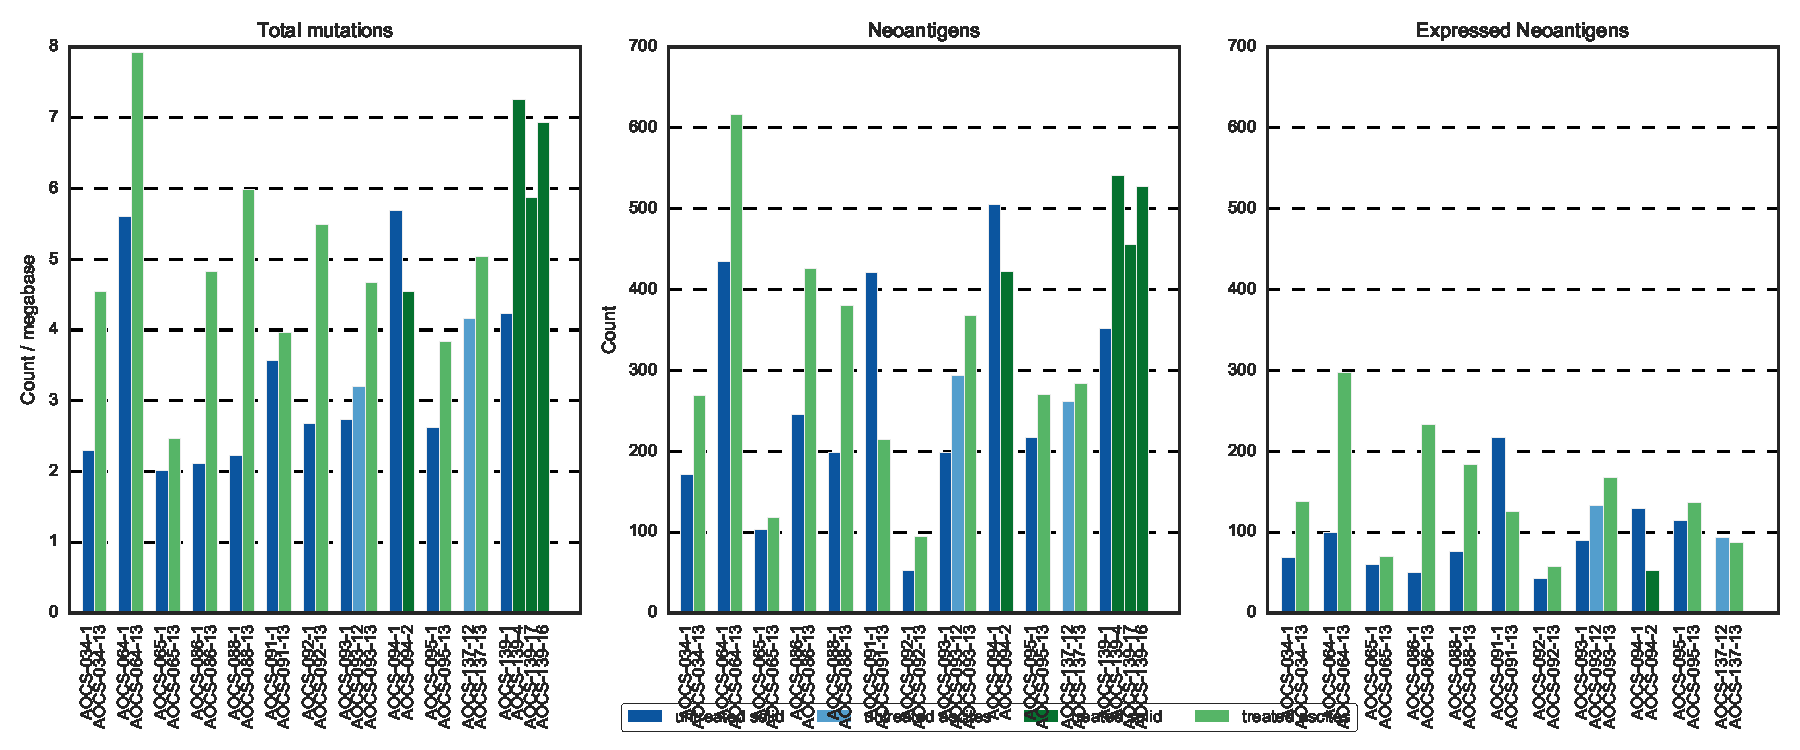
\includegraphics[scale=1.0]{figures/paired_counts.pdf}
\caption{Mutations, neoantigens, and expressed neoantigens for the patients with paired pre-/post-chemotherapy samples.}
\label{fig:supp_paired}
\end{figure}

\begin{comment}
\usetikzlibrary{fit,positioning}
\begin{figure}
\centering
\begin{tikzpicture}
\tikzstyle{main}=[rectangle, rounded corners, minimum size = 10mm, thick, draw =black!80, node distance = 10mm]
\tikzstyle{connect}=[-latex, thick]
\tikzstyle{box}=[rectangle, draw=black!100]
  \node[main] (coefficients) [label=above:Coefficients] { $\beta \sim \mathit{N}(0, 20)$ };
  \node[main] (globalmean) [right=of coefficients,label=above:Global Mean] { $\mu_\text{global} \sim \mathit{N}(0, 100) $ };
  \node[main] (patientsigma) [right=of globalmean,label=above:Patient Variance] { $\sigma_\text{patient} \sim \mathit{Cauchy}(0, 2) $ };
  \node[main] (samplesigma) [right=of patientsigma,label=above:Sample Variance] { $\sigma_\text{sample} \sim \mathit{Cauchy}(0, 2) $ };

  \node[main] (patientmean) [below=of globalmean, xshift=25mm] {$\mu_d \sim \mathit{N}(\mu_\text{global}, \sigma_\text{patient}) $};

  \node[main] (mu) [below=of patientrmean,label=below:] { $\mu_i = \mu_d + \beta \cdot x_i $ };
  \node[circle, thick, draw=black!80] (data) [left=10mm of mu,label=above:Observed] { $x_i$ };

  \node[main] (y) [below=of mu] {$\log y_i \sim \mathit{N}(\mu_i, \sigma_{sample})$};
  \node[circle, thick, draw=black!80] (obsy) [left=5mm of y,label=above:Observed] { $y_i$ };

  \path (globalmean) edge [connect] (patientmean)
        (patientsigma) edge [connect] (patientmean)
        (coefficients) edge [connect] (mu)
        (data) edge [connect] (mu)
        (obsy) edge [connect] (y)
        (patientmean) edge [connect] (mu)
        (mu) edge [connect] (y)
        (samplesigma) edge [connect] (y);

  \node[rectangle, inner sep=8mm,fill=gray!100, draw=black!100, fill opacity=0.2, fit= (patientmean) (y) (data) ,yshift=-3mm,xshift=1mm,label=below:$d \in \text{patients}$] {};
  \node[rectangle, inner sep=6mm,fill=gray!100, draw=black!100, fill opacity=0.2, fit= (mu) (y) (data),yshift=1mm,xshift=1mm,label=below:$i \in \text{samples($d$)}$] {};


\end{tikzpicture}
\caption{Bayesian model architecture for paired samples. For unpaired samples, $\mu_d$ is set to $\mu_\text{global}$. Three models were fit separately, using the same predictive variables $x_i$ but setting the predicted variable $y_i$ to the number of mutations, the number of neoantigens, and the number of expressed neoantigens in a sample $i$. The $x_i$ were whether the sample was chemotherapy-treated (binary), whether it was low purity (binary -- low purity taken to be the bottom quartile of the AOCS purity estimate from qPure~\cite{Song_2012}), whether the tissue type was ascites (binary), the number of samples from the same patient (integer), and an interaction variable that was 1 if the sample was both solid tumor and treated, and otherwise 0 (binary).}
\label{fig:model_architecture}
\end{figure}
\end{comment}


\begin{comment}
\begin{figure}[htbp]
\centering
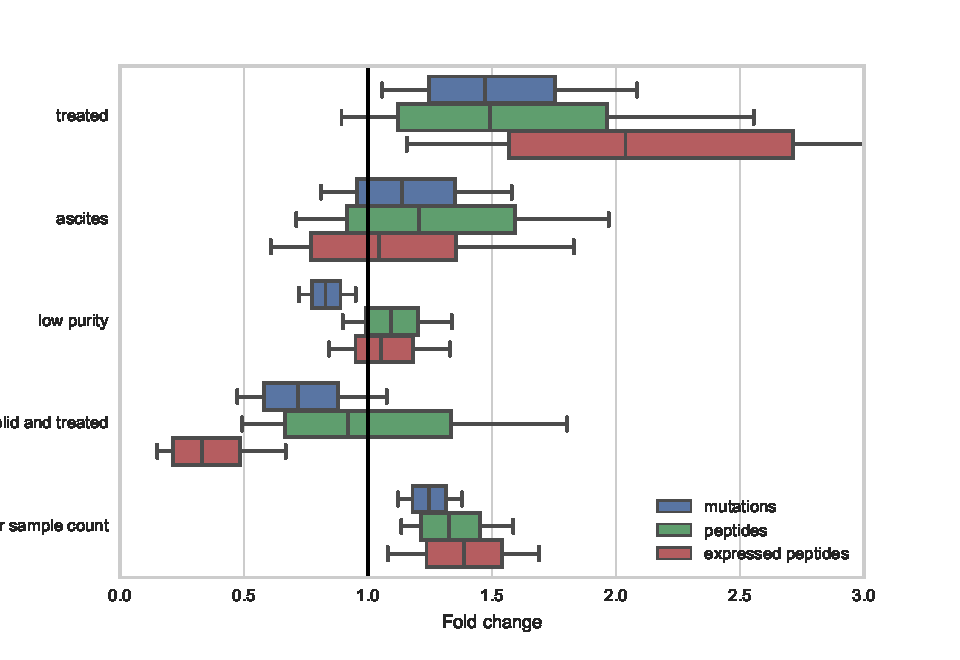
\includegraphics[scale=1.0]{figures/bayesian_model_effects.pdf}
\caption{Bayesian model effects. }
\label{fig:bayesian_model_effects}
\end{figure}

\begin{figure}[htbp]
\centering
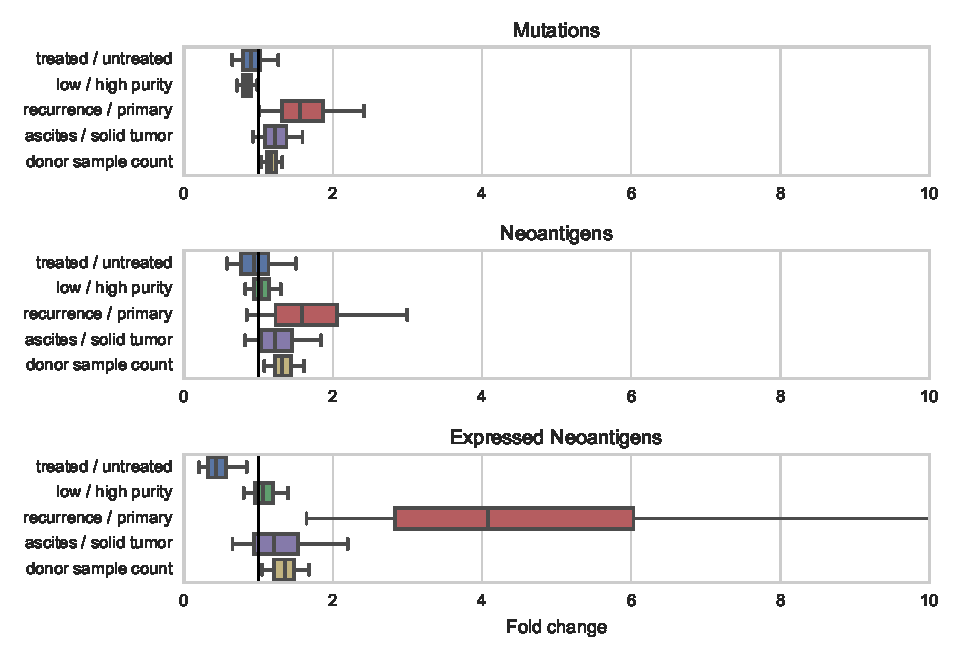
\includegraphics[scale=1.0]{figures/bayesian_model_effects_separate.pdf}
\caption{Parameter estimates for a model separating treatment effect from recurrence/relapse time-point. The architecture is the same as in Figure~\ref{fig:model_architecture}. This model had high uncertainties and its results are not reported in the paper.}
\label{fig:bayesian_model_effects_separate}
\end{figure}
\end{comment}



\begin{figure}
\centering
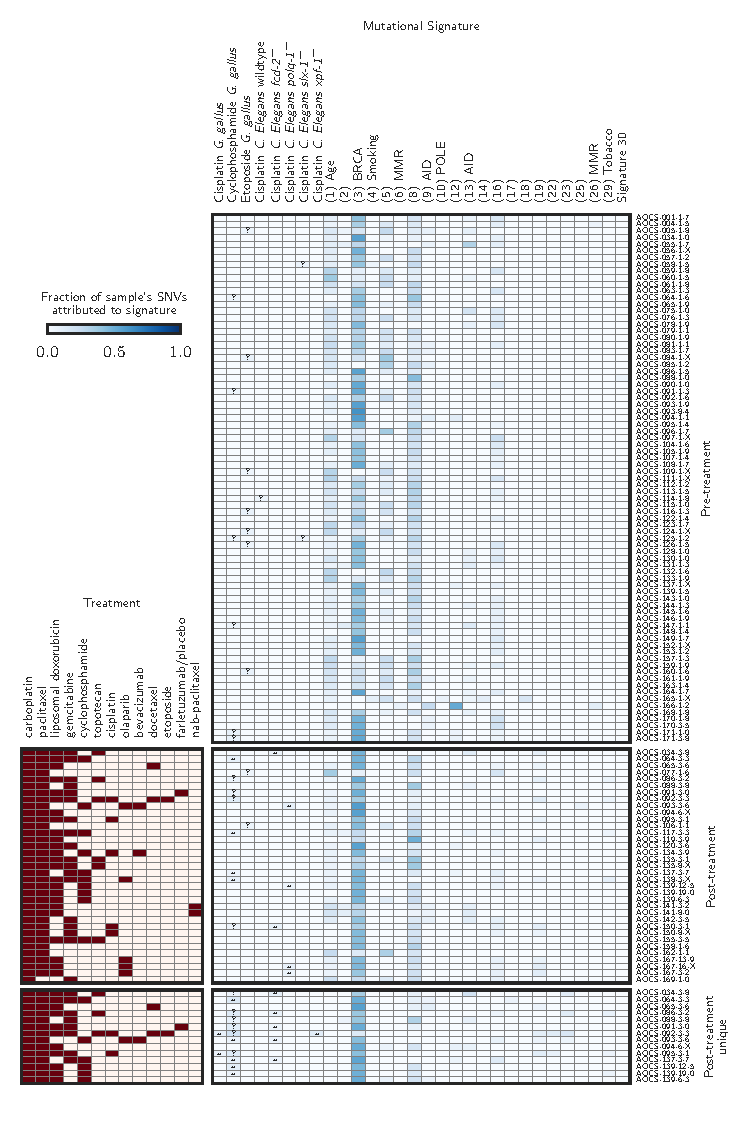
\includegraphics[scale=1.0]{figures/supplementary_signatures.pdf}
\caption{\textbf{Mutational signature deconvolutions for all samples.} The symbols are as in main text figure~\ref{fig:signatures}.}
\label{fig:supp_signatures}
\end{figure}

\begin{figure}
\centering
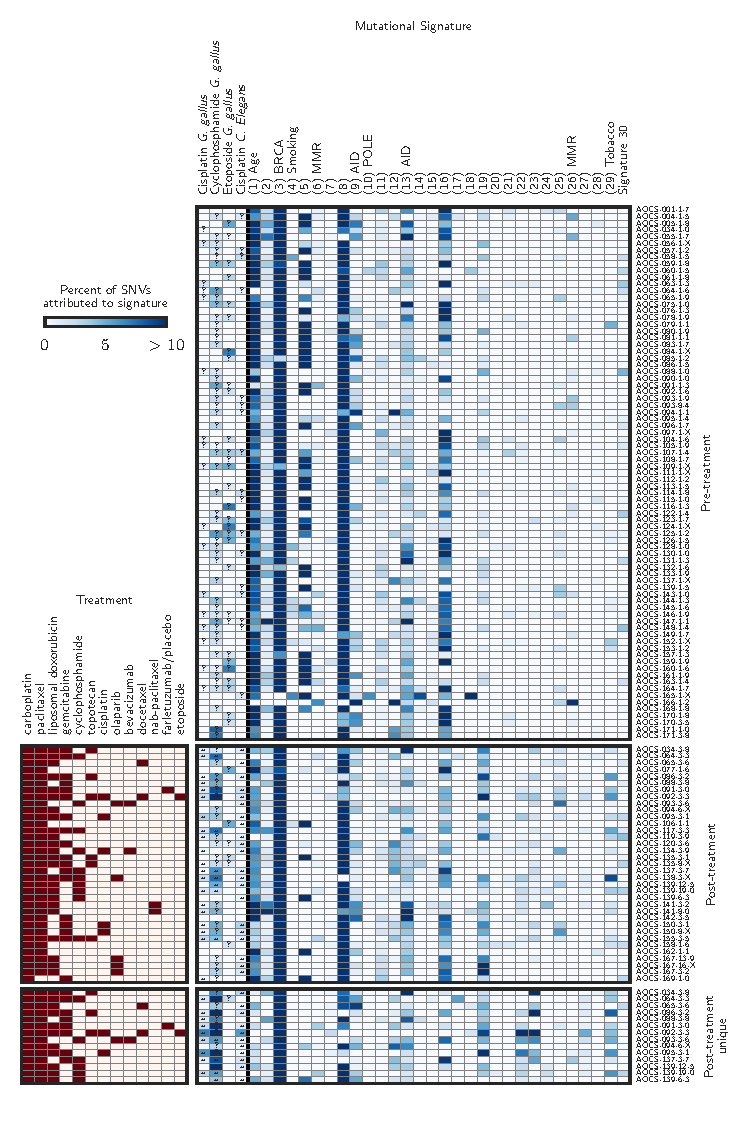
\includegraphics[scale=1.0]{figures/supplementary_signatures_no_cutoff.pdf}
\caption{\textbf{Mutational signature deconvolutions for all samples, without any minimum threshold.} The symbols are as in main text figure~\ref{fig:signatures}.}
\label{fig:supplementary_signatures_no_cutoff.pdf}
\end{figure}

\begin{comment}
\begin{figure}
\centering
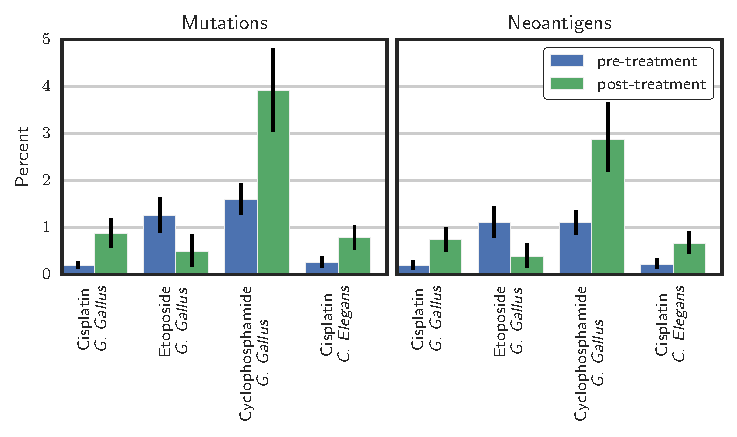
\includegraphics[scale=1.0]{figures/sources_of_mutations_and_neoantigens_ungrouped.pdf}
\caption{\textbf{Contributions of chemotherapy-associated mutational signatures to mutations and neoantigens, as a fraction of total.}}
\label{fig:supp_sources}
\end{figure}
\end{comment}


\begin{figure}
\centering
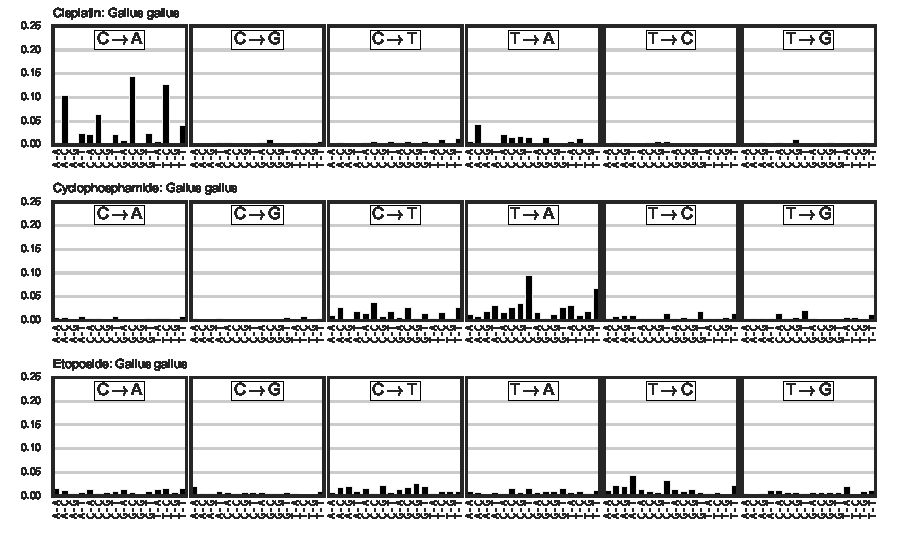
\includegraphics[scale=1.0]{figures/extracted_signatures_chicken.pdf}
\caption{Mutational signatures extracted from Szikriszt et al.~\cite{Szikriszt_2016}}
\label{fig:supp_extracted_signatures_chicken}
\end{figure}

\begin{figure}
\centering
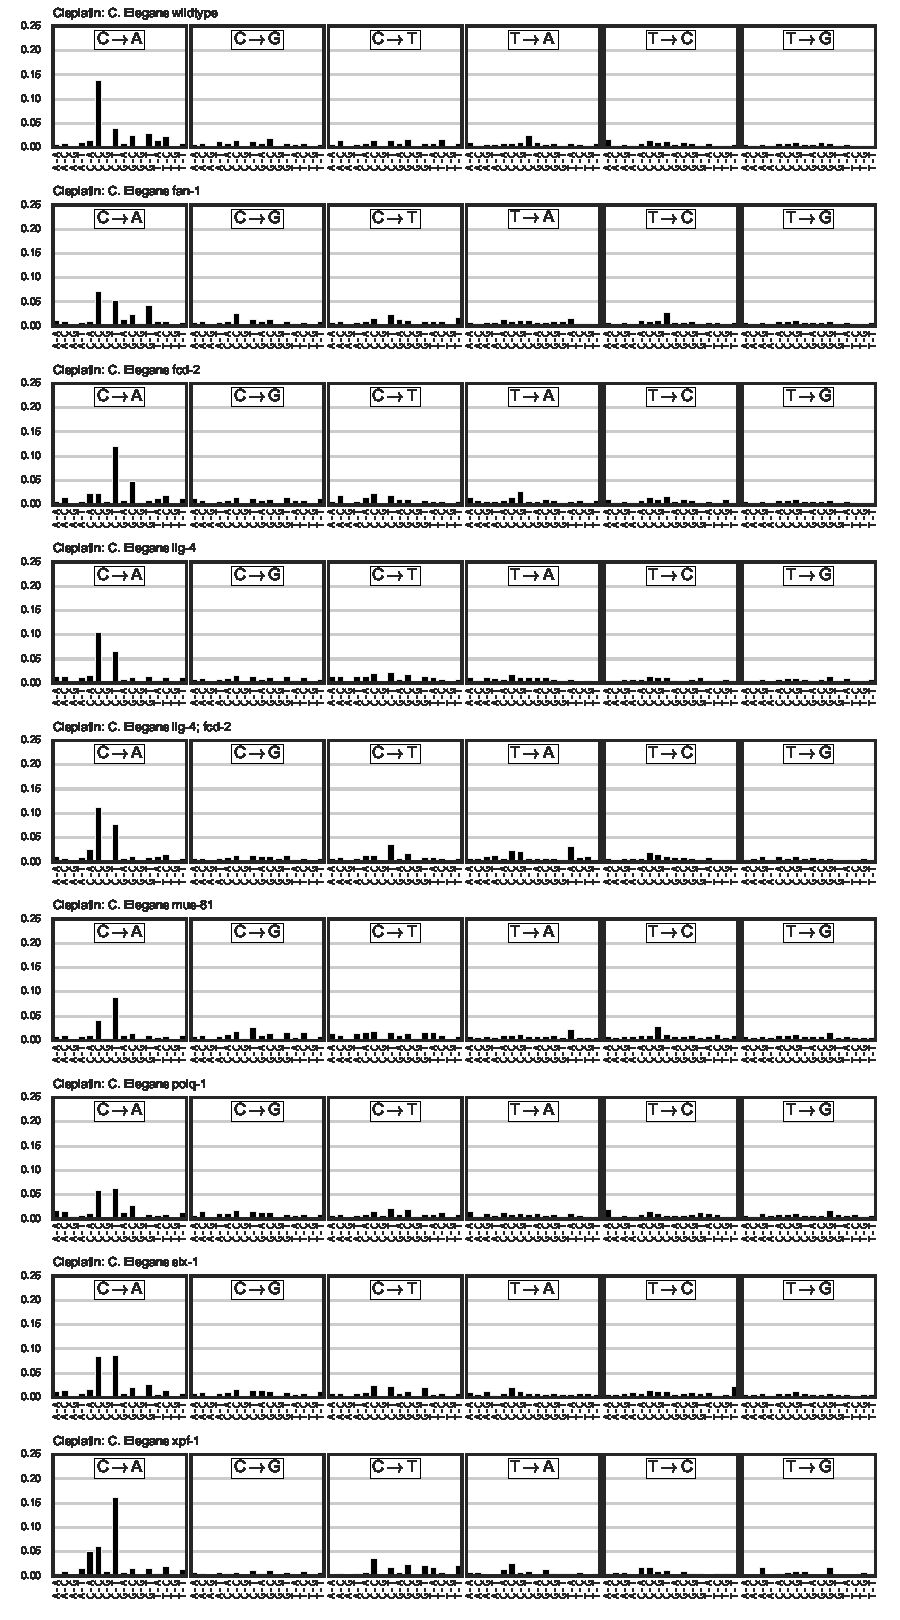
\includegraphics[scale=1.0]{figures/extracted_signatures_worm.pdf}
\caption{Mutational signature extracted from Meier et al.~\cite{Meier_2014}}
\label{fig:supp_extracted_signatures_worm}
\end{figure}

\FloatBarrier
